% This is a template for your written document.
%
% To compile using latexmk on the command line, run the following: 
% latexmk -pdf main.tex

\documentclass[12pt]{article}
\usepackage{setspace}
\usepackage{graphicx} % used for includegraphics
\singlespace
\usepackage[left=1in,right=1in,top=1in,bottom=1in]{geometry}

\title{\textbf{Using Machine Learning (XGBoost) Methods to Analyze Traffic Flows in Lima, Peru}}
\author{Ellery Park}

\begin{document}

\maketitle

As the global population grows exponentially, an increasing proportion of the world has begun to live in
urban environments, with an estimated 68\% predicted to live in cities by 2050~\cite{UN_DESA}. Accurate traffic flow prediction models are necessary 
to optimize traffic control systems and inform sustainable, safe, and cost-effective infrastructure. Recent advances in machine learning (ML) and deep learning techniques 
enhance Intelligent Transportation Systems (ITS) by more accurately predicting traffic flows than historical averages or linear regression techniques~\cite{app15073866}. 
However, the majority of studies concentrate on highly-developed cities where data is readily available, while fewer studies
focus on the implementation of ML-powered traffic control monitoring systems in developing cities~\cite{Dorosan}. Since developing cities are
likely to suffer from uneven development which begets traffic congestion and traffic-related accidents, understanding traffic
flows in developing cities is crucial for policymakers and urban planners.

This project aims to create a dynamic traffic flow model of Lima, Perú, utilizing Extreme Gradient Boosting (XGBoost) and Random Forest (RF) machine learning techniques.
XGBoost and RF were chosen due to their relatively low computational requirement compared to deep learning neural networks,
their high performance with limited data, and their proficiency with tabular data. Open-Source Map (OSM) data will be used to generate a road map of the city, 
while additional open-source data from the Autoridad de Transporte Urbano (ATU),
Indicadores Mensuales de Tráfico, and TomTom will be used to model population flows according to spaciotemporal indicators.
Feature importance analysis will be applied to determine the impact of each feature on the traffic outcome.
The end product will be a model created using GIS software that can predict traffic flows given certain conditions, such as time, date, and
weather. The model will additionally be able to generate predictive outcomes of road closures or the construction of new routes. A potential GUI for the software 
is displayed in Figure ~\ref{fig:gui}.

The project is informed by a variety of machine learning research initiatives which applied machine learning techniques to analyze 
traffic in urban environments across the globe. A variety of studies have displayed the effectiveness of XGBoost and RF
in modeling traffic flows in developing countries compared to ANN, LSTM, or SVM deep learning models \cite{Dorosan, ABDULRASHID2025103969, en18071685, HAMMOUMI2025813}. 
Feature importance analyses are applied in Abdulrashid et al. \cite{ABDULRASHID2025103969}, and in 
Dorosan et al. \cite{Dorosan}, which use a variety of Shapley's additive explanation (SHAP), PFI, and FIRM scores to compare the behvaiors
of various models.
The GIS mapping aspect of the project is inspired by a study in Ali Menjeli, Algeria, which combines LSTM-analyzed data to create isochromes that are
mapped using GIS software \cite{Fenghour2025}. 


\begin{figure}[h]
\begin{center}
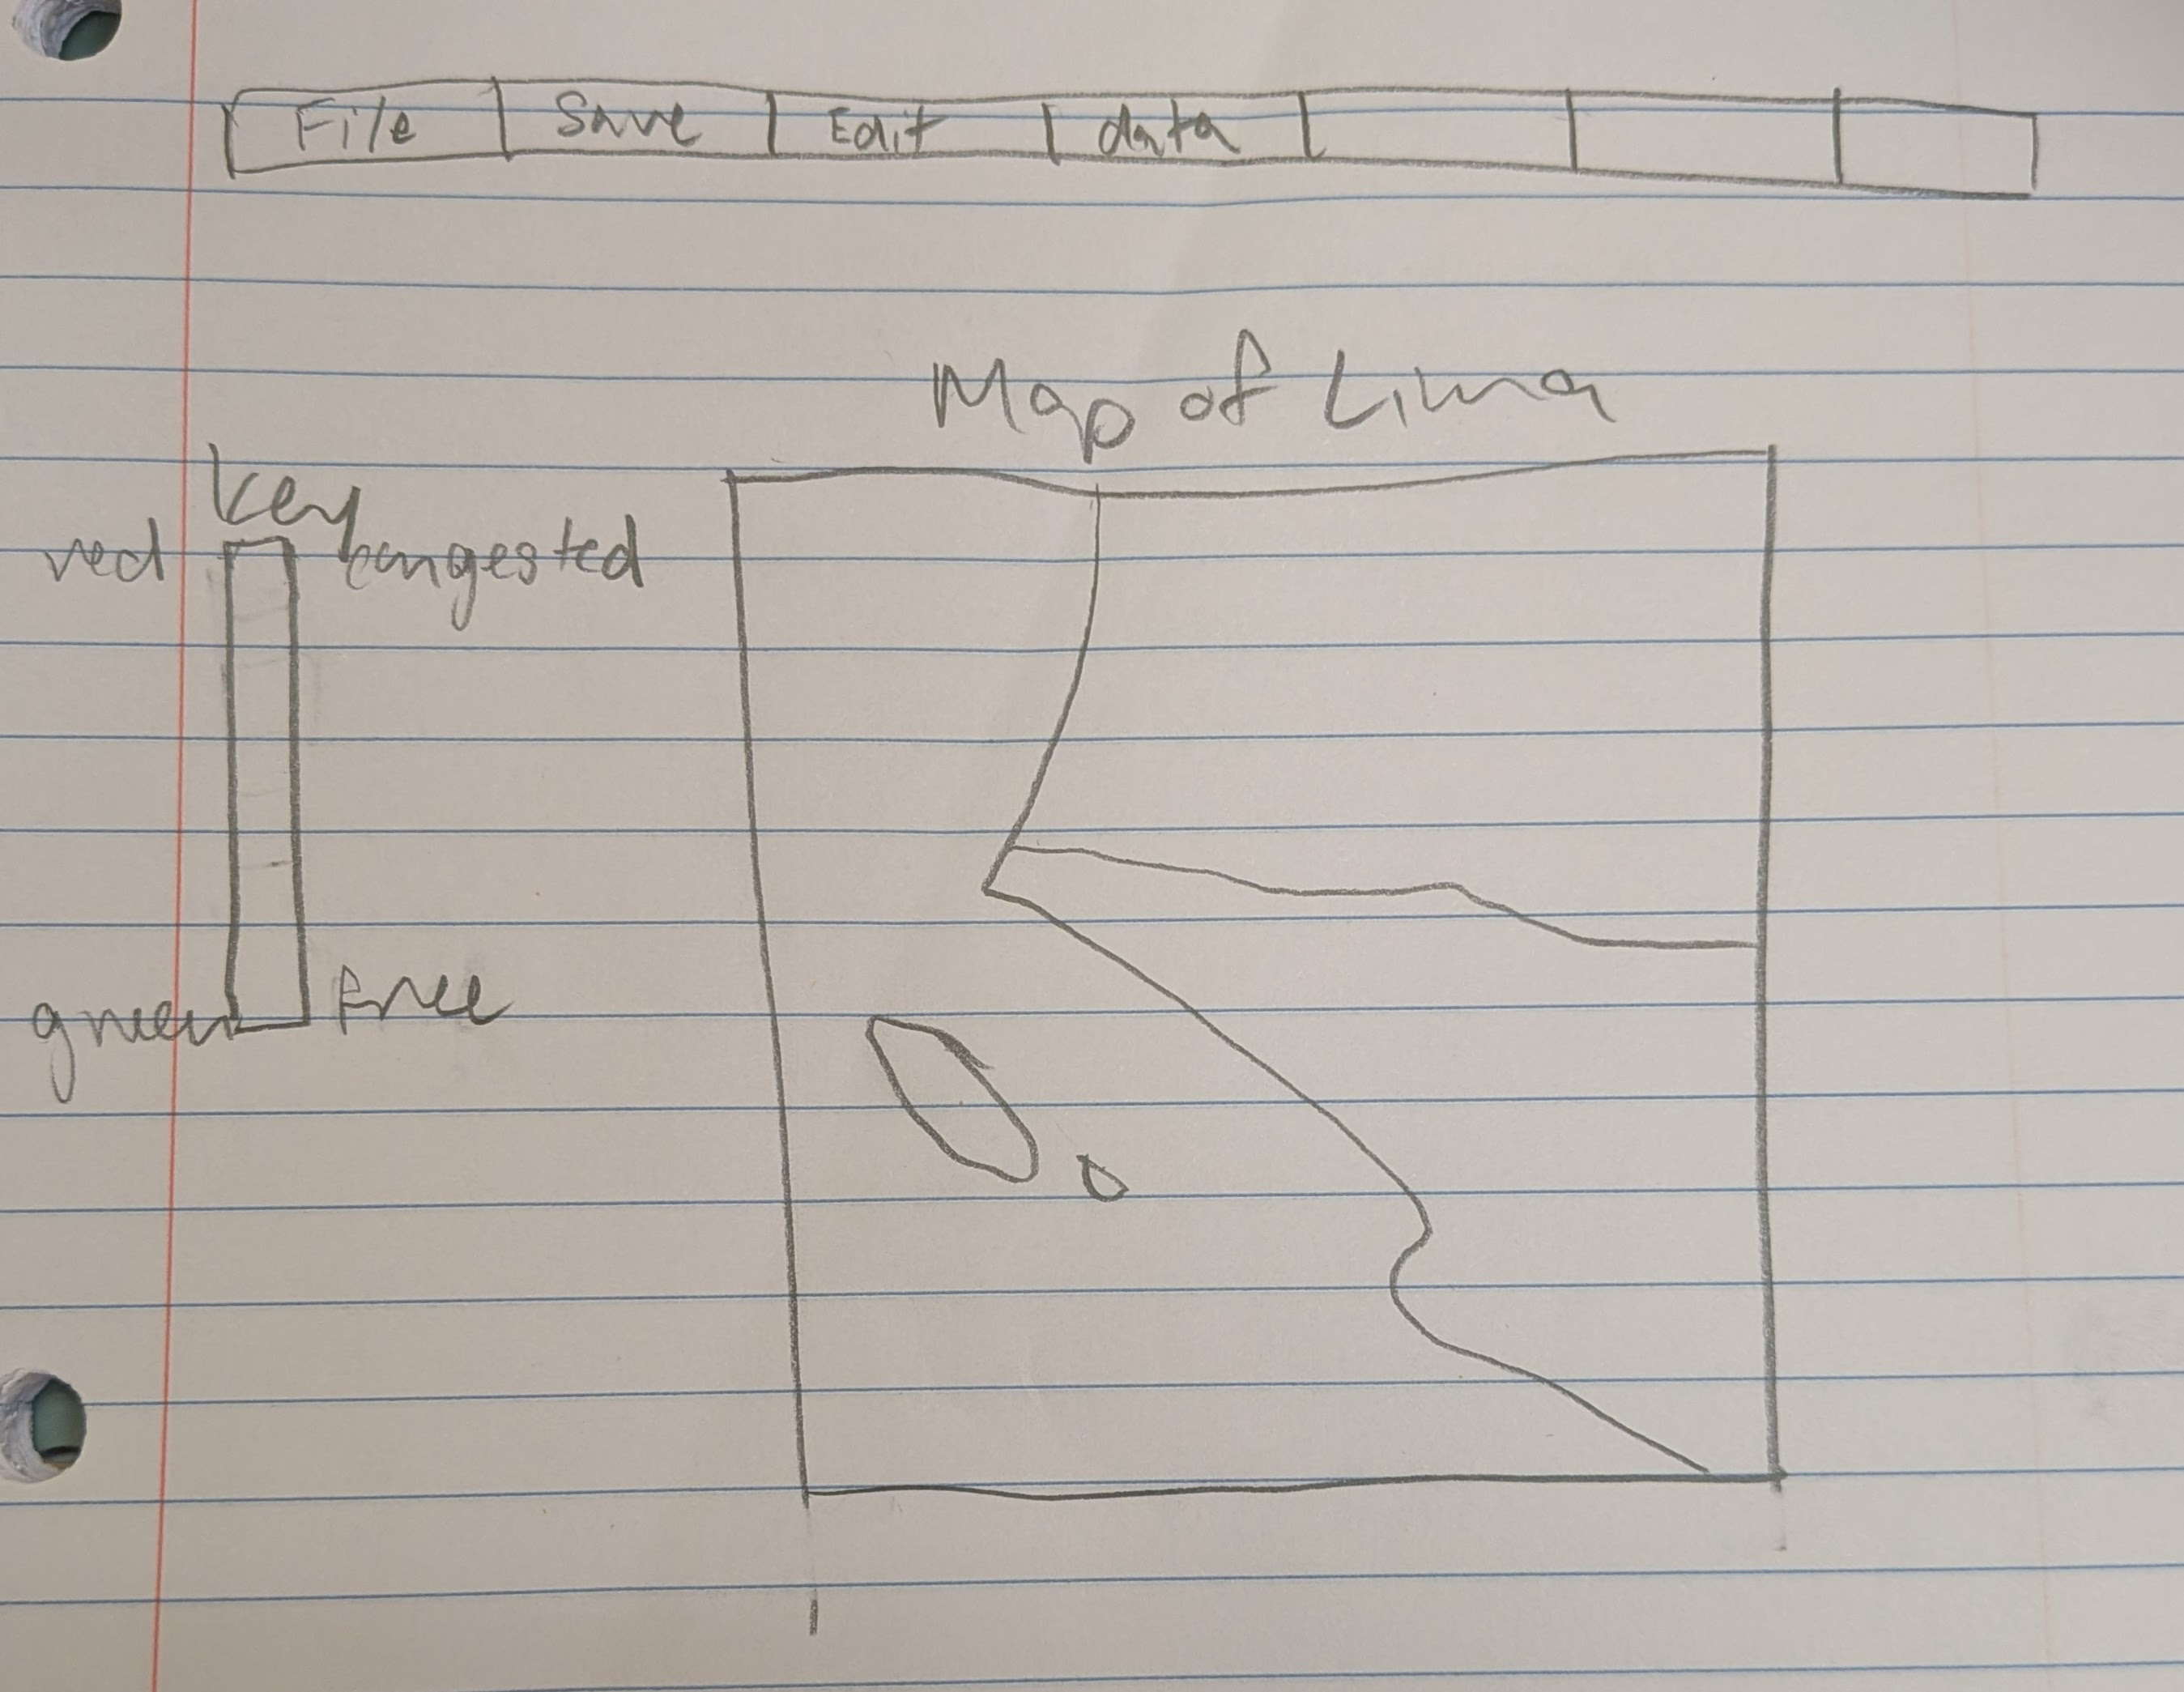
\includegraphics[scale=0.1]{proposed_gui.jpg}
\caption{A hand-drawn GUI of the final traffic-mapping software.}
\label{fig:gui} 
\end{center}
\end{figure}


\newpage
\section*{Appendix}
Product features.
\begin{itemize}
	\item Creation of pre-processed data tables (5 hours)
	\item Visualization of the statistical baseline (found using historical average \ linear regression techniques) (2.5)
	\item Table of XGBoost results. (time to implement 3; time to run/ tune - two weeks)
	\item Table of RF results. (2 weeks)
	\item Map results to GIS software to create a color-coded visualization of congestion on each street. (8 hrs)
	\item Plot to display the importance of each feature on the outcome (calculated using SHAP, PFI, and/or FIRM). (2 hours)
	\item Loss plot to determine the accuracy of each model. (2 hours)
	\item Hypothetical: Create software that will generate color-coded maps of Lima based on certain parameters. (10)
	\item Implement capacity of GIS model to vary depending on time, date, and weather features. (4)
	\item Implement capacity of GIS model to respond to conditions such as a closed road or or an additional freeway. (4)
\end{itemize}
~30 hrs + 2 weeks?

\nocite{*}

\bibliographystyle{acm}
\bibliography{bibliography.bib}

\end{document}
